\subsection*{Aufgabe 7 - Resultat und Visualisierung}

Animiert wird die Bewegung des Knickarmroboters mithilfe des \texttt{plot} Befehls. Hierfür werden die bereits in Aufgabe 1 erläuterten homogenen Transformationsmatrizen genutzt, um die generalisierten Koordinaten $\alpha$ und $\beta$ auf kartesische Koordinaten zu übersetzen. Das erste Gelenk ist hierbei gelb, das zweite grün eingefärbt. Die Zielposition ist mit einem orangenem Kreis markiert. Ein einzelnes Frame ist in Abbildung \ref{fig:visualisierung} zu sehen. Erzeugt wird diese Animation mit dem in Listing \ref{lst:animation} dargestellten Code. Welche \texttt{drawnow} ausnutzt und für jedes Frame eine Pause einlegt, um die adaptive Schrittweite des Runge-Kutta solvers auszugleichen. Die Funktion \texttt{plot\_robot} erzeugt die eingefärbten Gelenke.

\begin{figure}[H]
    \centering
    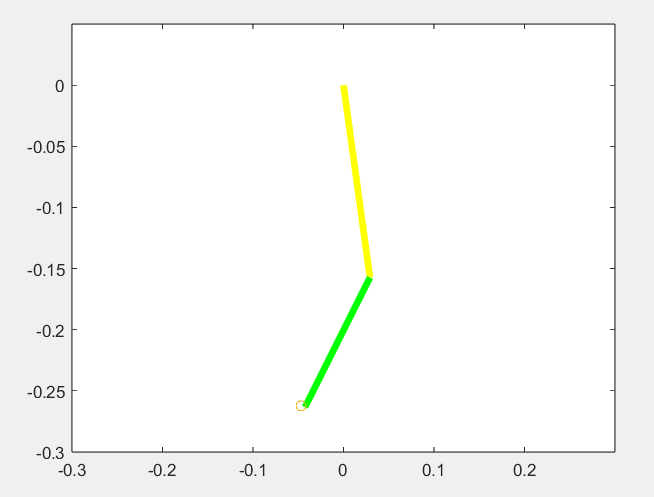
\includegraphics[width=0.8\linewidth]{img/visualisierung.png}
    \caption{Visualisierung der Simulation}
    \label{fig:visualisierung}
\end{figure}




\begin{lstlisting}[caption={Definition der rechten Seite},label={lst:animation}]
    %% Visualization
if plot_Ergebnis
    alphas = y(:, 1);
    betas = y(:, 3);
    [T_02, T_03] = dh_trafo();
    orig = [0 0 0 1]';
    time = [diff(t); 0];
    
    % Animation
    figure(1);
    % plots maximal 250 frames
    max_frame = 250;
    n_frame = min(size(y,1), max_frame);
    for frame=1:n_frame
        i = floor(frame/n_frame .* numel(t));
        G2 = T_02(alphas(i), betas(i))*orig;
        G3 = T_03(alphas(i), betas(i))*orig;
        plot_robot(G2, G3)
        hold on
        plot(y_end_glob(1), y_end_glob(2), "o")
        hold off
        drawnow;
        %wait such that the animation is as long as the simulated time
        pause(time(i));
    end
end
\end{lstlisting}




\subsection*{Diskussion}